\documentclass[10pt]{article}
\usepackage[margin=0.85in]{geometry}
\usepackage{tikz}
\usepackage{amsmath}
\usepackage{booktabs}
\usepackage{array}
\usepackage{longtable}
\usepackage{xcolor}
\usepackage{underscore}
\usepackage[hidelinks]{hyperref}
\usetikzlibrary{positioning,arrows.meta,fit,backgrounds,calc}

\definecolor{cif}{HTML}{dceef9}
\definecolor{core}{HTML}{e2efd6}
\definecolor{util}{HTML}{f5efe0}
\definecolor{back}{HTML}{f4dede}
\definecolor{cfg}{HTML}{efe6fb}

\newcommand{\sig}[1]{\texttt{\small #1}}
\newcommand{\blk}[1]{\textbf{#1}}
\newcolumntype{P}[1]{>{\raggedright\arraybackslash}p{#1}}

\title{\textbf{RMC --- MC-Core Block Reference}\\[2pt]
\large sub-block structure, I/O ports, and functions}
\author{Reconfigurable Memory Controller (DDR1--5), one channel per core}
\date{\today}

\begin{document}
\maketitle
\vspace{-1.2em}

\noindent This reference reflects the current RTL (\sig{rtl/cif}, \sig{rtl/utils}, \sig{rtl/mc},
\sig{rtl/rtl_pkg_config}, \sig{rtl/csr_config}). Built blocks list real ports; not-yet-RTL blocks
are described at block level. One MC core per DDR channel; channel select is extracted in the CIF.

%====================================================================
\section{Top spine}
\begin{center}
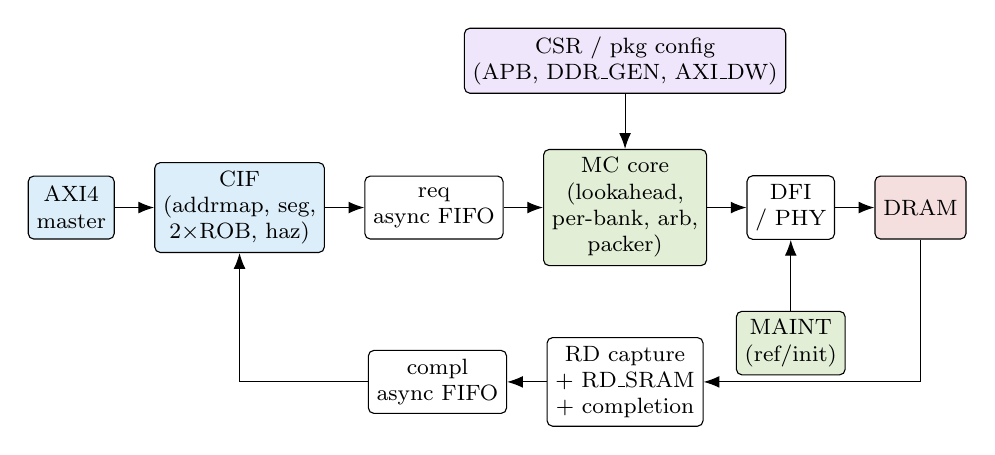
\begin{tikzpicture}[font=\footnotesize,
  node distance=5mm,
  b/.style={draw,rounded corners=2pt,minimum height=8mm,align=center,inner sep=3pt},
  cif/.style={b,fill=cif}, core/.style={b,fill=core}, back/.style={b,fill=back},
  cfg/.style={b,fill=cfg}, a/.style={-{Latex[length=2mm]}}]
\node[cif] (axi) {AXI4\\master};
\node[cif,right=of axi] (cif) {CIF\\(addrmap, seg,\\2$\times$ROB, haz)};
\node[b,right=of cif,fill=white] (af1) {req\\async FIFO};
\node[core,right=of af1] (core) {MC core\\(lookahead,\\per-bank, arb,\\packer)};
\node[b,right=of core,fill=white] (dfi) {DFI\\/ PHY};
\node[back,right=of dfi] (dram) {DRAM};
\draw[a] (axi)--(cif); \draw[a] (cif)--(af1); \draw[a] (af1)--(core);
\draw[a] (core)--(dfi); \draw[a] (dfi)--(dram);
% return path
\node[b,below=9mm of core,fill=white] (rd) {RD capture\\+ RD_SRAM\\+ completion};
\node[b,left=of rd,fill=white] (af2) {compl\\async FIFO};
\draw[a] (dram.south) |- (rd.east);
\draw[a] (rd)--(af2); \draw[a] (af2.west) -| (cif.south);
% side blocks
\node[cfg,above=7mm of core] (cfg) {CSR / pkg config\\(APB, DDR_GEN, AXI_DW)};
\node[core,below=9mm of dfi] (me) {MAINT\\(ref/init)};
\draw[a] (cfg)--(core); \draw[a] (me.north)--(dfi.south);
\end{tikzpicture}
\end{center}

\noindent Forward: \sig{AXI $\to$ CIF $\to$ req async FIFO $\to$ lookahead $\to$ bank-dec $\to$
per-bank cell $\to$ arb $\to$ packer $\to$ DFI $\to$ DRAM}. Return: \sig{DRAM $\to$ RD capture $\to$
RD_SRAM $\to$ completion $\to$ compl async FIFO $\to$ CIF}. Only true CDC = CIF$\leftrightarrow$MC
(the two async FIFOs); DFI seam is same-clock.

%====================================================================
\section{Compile-time config (\texttt{rmc\_cfg\_pkg})}
One DDR generation per build (\sig{DDR_GEN}). Everything parametric.
\begin{longtable}{P{3.2cm} P{3.0cm} P{8.0cm}}
\toprule
\blk{param} & \blk{value (DDR5)} & \blk{meaning}\\ \midrule \endhead
\sig{DDR_GEN} & \sig{DDR5} & build-time generation select (DDR1--5)\\
\sig{N_RANKS} & 2 & ranks (lanes); fully duplicated state, shared issue\\
\sig{N_BG / N_BANK_PER_BG} & 8 / 4 & bank groups / banks per group (= 32 banks/rank)\\
\sig{ROW_W / COL_W} & 18 / 10 & row / column address widths\\
\sig{BL / DQ_W} & 16 / 32 & burst length / sub-channel data width\\
\sig{PKT_BYTES} & 64 & packet = \sig{BL*DQ_W/8} = one 64\,B line = one CAS\\
\sig{N_CH} & 2 & DDR channels (one MC core each)\\
\sig{DDR_CHANNEL_W} & \sig{2*DQ_W}=64 & data width per DDR channel\\
\sig{AXI_DW} & \sig{N_CH*DDR_CHANNEL_W} & \textbf{matched BW} (see \S\ref{sec:axi})\\
\sig{P_MAX} & 4 & packets per bank (row-hit train); sets bank queue depth\\
\sig{BANK_Q_DEPTH} & \sig{P_MAX}=4 & per-bank TCAM / cas\_fifo depth\\
\sig{DADDR_W} & 34 & \sig{\{rank,bg,bank,row,col\}} DRAM-coord width\\
\bottomrule
\end{longtable}

%====================================================================
\section{Address map (STAGE 24)}
Pure field-slice, no hash (\sig{rmc\_cif\_addrmap}). Consecutive packets rotate BGs
(diff-BG CAS $=t_{CCD\_S}=8$, writes safe), then \sig{col_lo} revisits a bank's next column = row-hit.

\noindent\textbf{Interleave (LSB$\to$MSB):}
\sig{offset[5:0] | ch | rank | BG_lo(rot) | col_lo(=P) | BG_hi | bank | col_hi | row}.

\begin{center}\footnotesize
\begin{tabular}{llll llll}
\toprule
request & packets & /ch & /(ch,rank) & banks & P/bank & cols (row-hit)\\ \midrule
4\,KB (MAX) & 64 & 32 & 16 & 4 & 4 & 4\\
2\,KB & 32 & 16 & 8 & 4 & 2 & 2\\
1\,KB & 16 & 8 & 4 & 4 & 1 & 1\\
64\,B & 1 & 1 & 1 & 1 & 1 & 1\\
\bottomrule
\end{tabular}
\end{center}

\noindent\sig{rmc\_cif\_addrmap} ports: \sig{sys_addr $\to$ daddr\{rank,bg,bank,row,col\}},
\sig{ch} (route to per-channel core), \sig{offset} (byte-in-packet, write mask).

%====================================================================
\section{CIF --- client interface}
Between AXI4 and the MC async FIFOs. Owns address map, segmentation, two ROBs, and the
same-line hazard interlock. Completion never back-pressures (\sig{ready} tied high).

\subsection{\texttt{rmc\_cif} (top)}
\begin{longtable}{P{4.2cm} P{1.3cm} P{9.0cm}}
\toprule
\blk{port} & \blk{dir} & \blk{function}\\ \midrule \endhead
\sig{aclk, aresetn} & in & AXI clock / async reset\\
\sig{aw*/w*/b* AXI4} & io & write address / data / response channels\\
\sig{ar*/r* AXI4} & io & read address / data channels\\
\sig{async_mc_req_*} & out & req stream to MC (rob\_index, op, daddr, pkt\_num, last\_in\_txn, sram\_slot)\\
\sig{async_mc_cmpl_*} & in & completion from MC (rob\_index, pkt\_num, status); ready tied high\\
\sig{wdb_we/waddr/wdin} & out & WD\_SRAM write port (CIF writes W beats)\\
\sig{rdb_re/raddr/rdout} & out/in & RD\_SRAM read port (CIF drains to R)\\
\bottomrule
\end{longtable}

\subsection{Sub-blocks}
\begin{itemize}\itemsep1pt
\item \blk{rmc\_cif\_addrmap} --- byte addr $\to$ daddr + ch + offset (\S3).
\item \blk{rmc\_cif\_seg} --- burst $\to \le$16-beat packets, narrow/WSTRB flag (stub).
\item \blk{rmc\_cif\_rob} ($\times$2, \sig{r\_rob}/\sig{w\_rob}) --- order via pointer shift-reg,
index-mapped backing stores (addr TCAM, inflow/outflow counters, cold meta). Addr-TCAM search
port probed by the opposite ROB.
\item \blk{rmc\_cif\_haz} --- RAW+WAR interlock. 1-cycle hits latch a stall on the requester's
slot; released when the matched older entry retires. WAW impossible (AXI write ordering).
\end{itemize}

\noindent\textit{\texttt{rmc\_cif\_haz} ports:}
\begin{longtable}{P{3.6cm} P{1.3cm} P{9.6cm}}
\toprule \blk{port} & \blk{dir} & \blk{function}\\ \midrule \endhead
\sig{clk, rst_n} & in & stateful (latched stalls)\\
\sig{raw_hit, raw_rd_ptr} & in & new read overlaps older write; new read's slot to hold\\
\sig{raw_wr_ptr} & in & matched older write slot (release key)\\
\sig{war_hit, war_wr_ptr, war_rd_ptr} & in & symmetric WAR\\
\sig{wr_free_vld/ptr, rd_free_vld/ptr} & in & retire pulses -> release matching stalls\\
\sig{r_stall_vector, w_stall_vector} & out & held per-entry stall bits to the two ROBs\\
\bottomrule
\end{longtable}

%====================================================================
\section{Utility library (\texttt{rtl/utils})}
Generic, parametric, standalone.

\begin{longtable}{P{3.0cm} P{12.0cm}}
\toprule \blk{module} & \blk{function + ports}\\ \midrule \endhead
\sig{rmc_fifo} & sync FIFO (count-based). Params \sig{WIDTH,DEPTH,FWFT,AF/AE_THRESH,PROT}.
Ports: \sig{clk,rst_n, wr_en,wr_data, rd_en,rd_data,rd_valid, full,empty,almost_*,count,overflow,underflow}.\\
\sig{rmc_sram} & 1W+1R RAM. Params \sig{WIDTH,DEPTH,RD_LAT(0/1/2),COLLIDE}. \sig{RD_LAT=0}=comb (0th-clk),
write-first. Ports: \sig{clk, we,waddr,wdata, re,raddr,rdata}.\\
\sig{rmc_regfile} & flop array, 1 write + N comb read ports, write-first bypass. Ports:
\sig{clk,rst_n, we,waddr,wdata, raddr[N_RD],rdata[N_RD]}.\\
\sig{rmc_async_fifo} & dual-clock Gray-pointer CDC FIFO. Ports: \sig{wclk,wrst_n,wr_en,wr_data,wfull,walmost_full,
rclk,rrst_n,rd_en,rd_data,rd_valid,rempty,ralmost_empty}.\\
\sig{rmc_lookahead} & bank-stall bypass window (below).\\
\bottomrule
\end{longtable}

\subsection{\texttt{rmc\_lookahead} --- bank-stall bypass window}
DEPTH-entry age-ordered window. Oldest-\emph{eligible} (\sig{valid \& rdy_vec[adr]}) issues, so a
younger packet to a ready resource bypasses a stalled older one; same-resource order held by the
shared ready bit. Payload in reg (\sig{PAYLOAD_IN_REG=1}) or in a comb-read meta store
(\sig{rmc_sram RD_LAT=0}, write-first) + free-list. Same-cycle arrive+issue: \sig{din} issues live
(bypass), not stored; the \sig{wr_ptr==rd_ptr} compare (internal to the write-first store) picks live
vs stored.
\begin{longtable}{P{3.2cm} P{1.3cm} P{9.8cm}}
\toprule \blk{port} & \blk{dir} & \blk{function}\\ \midrule \endhead
\sig{clk, rst_n} & in & \\
\sig{din_valid/rdy_out} & in/out & ingress handshake (rdy = window has room)\\
\sig{din_adr} & in & resource key (probes \sig{rdy_vec}); = \{bg,bank\}\\
\sig{din_payload} & in & wide payload (= \{r/w,row,col,mem\_ptr\})\\
\sig{rdy_vec[N_RDY]} & in & per-resource ready (= bank\_rdy)\\
\sig{out_valid/ready} & out/in & egress handshake\\
\sig{out_adr, out_payload} & out & issued packet\\
\bottomrule
\end{longtable}

%====================================================================
\section{Per-bank path (\texttt{rmc\_bank})}
One cell per \sig{\{rank,bank\}}. Open-page, single open row. Exploits the row-streaked arrival from
the address map: two comparators + a 1-bit toggle split the stream.
\begin{itemize}\itemsep1pt
\item \blk{CMP1} \sig{row == open_row} (\& \sig{state==OPEN}) $\to$ hit $\to$ \sig{cas_fifo}; else miss.
\item \blk{CMP2} \sig{row == last_miss_row} $\to$ \sig{new_row} flips the toggle; miss pushed to
\sig{row_miss_fifo} tagged with the toggle.
\item \blk{toggle} delimits per-row groups in \sig{row_miss_fifo}: drain pops while
\sig{toggle==head.toggle} = one row $\to$ one ACT, then CAS the group.
\item depths: \sig{cas_fifo = row_miss_fifo = BANK_Q_DEPTH = P_MAX = 4}.
\item FSM: \sig{IDLE $\to$ ACTING $\xrightarrow{t_{RCD}}$ OPEN $\xrightarrow{grant\_pre}$ PREING
$\xrightarrow{t_{RP}}$ IDLE}, plus \sig{REFING}. Issue edges start transitions; scoreboard \sig{can_*}
complete the transient states.
\end{itemize}
\begin{longtable}{P{3.6cm} P{1.3cm} P{9.6cm}}
\toprule \blk{port} & \blk{dir} & \blk{function}\\ \midrule \endhead
\sig{clk, rst_n} & in & \\
\sig{admit_valid/ready} & in/out & packet in from decoder (post-lookahead)\\
\sig{admit_row/col/op/sptr} & in & row, column, R/W, payload slot\\
\sig{can_act/cas/pre} & in & timing legality from scoreboard\\
\sig{ref_pending/ref_done} & in & maintenance refresh handshake\\
\sig{act_rdy/cas_rdy/pre_rdy} & out & command readiness to the arb tree\\
\sig{grant_act/cas/pre/ref} & in & arb grant (pop on CAS)\\
\sig{out_row/col/op/sptr} & out & issued-command payload to packer\\
\bottomrule
\end{longtable}

%====================================================================
\section{Back-end (planned RTL)}
Block-level; not yet implemented.
\begin{itemize}\itemsep1pt
\item \blk{SCOREBOARD} --- GC (CK counter), per-scope timing regs; \sig{next_* = GC + const};
comparator $\to$ \sig{can_*} (\sig{(GC-next)[MSB]}). Split by arb level (bank/BG/rank/global);
one shared \sig{TIMING_CONST} addend table. \sig{dqFree} gates CAS (cross-rank occupancy).
\item \blk{ARB} class-split lanes (cas/act/pre) per rank $\to$ L3 2:1-per-class across ranks
$\to$ N-winner phase bundle. Selection+fairness only (legality folded into \sig{can_*}).
\item \blk{PHASE_PACKER} --- gear 1:N, places the bundle (CA slot, $\le$1 CAS/8CK), sole FSM-commit
edge; arms the data engines at CAS-commit.
\item \blk{DATA} --- WL launcher + write splitter ($\leftarrow$ WD\_SRAM), RL line + read accumulator
($\to$ RD\_SRAM); deterministic shift lines, no CAM.
\item \blk{COMPLETION} --- merges rd\_done/wr\_done $\to$ tag-only \sig{\{rob_index,pkt_num,status\}}
$\to$ resp async FIFO.
\item \blk{MAINT} --- INIT + REFRESH (REFsb-preferred, debt counter), RFM/ZQ/MRW stubs; override-inject
into the packer, never CAS.
\end{itemize}

%====================================================================
\section{Matched-bandwidth AXI width}\label{sec:axi}
\[
\sig{AXI_DW} \;=\; \sig{N_DDR_CHANNELS}\times\sig{DDR_CHANNEL_WIDTH}
\]
so AXI ingress BW $=$ DDR egress BW $\Rightarrow$ WD/RD SRAM and ROB inflow/outflow stay balanced
(no buffer blow-up). Derived in the package, not a free per-instance parameter.

\noindent\textbf{Caveat:} bandwidth $=$ width $\times$ frequency, so the width-only form is exact
\emph{only} when \sig{aclk == DDR data rate}. If the clocks differ, scale:
\[
\sig{AXI_DW} \;=\; \sig{N_CH}\times\sig{DDR_CHANNEL_W}\times\frac{f_{ddr}}{f_{aclk}},
\]
else AXI bottlenecks and the buffers drift (\sig{CLK_RATIO} param = TODO). DDR sustained BW is
$\sim$60--85\% of peak, so AXI sized to peak is slightly over-provisioned --- DRAM stays the limiter.

\end{document}
